% !TeX root = ../main.tex

\section{Systems of Linear Equations: Direct Methods}
We are talking about
\begin{LARGE}
$$
    Ax=b\Leftrightarrow\begin{cases}
        a_{11}x_1+a_{12}x_2+\cdots+a_{1n}x_n=b_1\\
        a_{21}x_1+a_{22}x_2+\cdots+a_{2n}x_n=b_2\\
        \vdots\hspace{11.5em}\vdots\\
        a_{n1}x_1+a_{n2}x_n+\cdots+a_{nn}x_n=b_n\\        
    \end{cases}
$$
$$
A\in\mathbb{R}^{n\times n}\qquad x,b\in\mathbb{R}^{n}
$$
\end{LARGE}

\subsection{Cramer Method}
Reminder:
$$
x_i=\frac{\det(A_i)}{\det(A)}\qquad i=1,\cdots,n
$$
Problem: finding the determinants computationally intensive, reminder of the Laplace rule:
$$
\det(A)=
\begin{cases}
    a_n\qquad\text{if $n=1$}\\
    \sum_{j=1}^n(-1)^{i+j}a_{ij}\Delta_{ij}\qquad\forall\,\,i\qquad\Delta_{ij}=\det(A_{ij})
\end{cases}
$$
Where $A_{ij}$ is the submatrix obtained by removing the $i$th row and $j$th column.\\On average we peform a number of operations equal to $3(n+1)!$, absolutely unfeasible, we must move to numerical counterparts/approximations.

\subsection{Numerical Approximations: Direct Methods}
We will talk about:
\begin{enumerate}[1)]
    \item Direct methods (fixed number of steps to get the solution, no notion of convergence)
    \item Iterative methods (non-ending number of steps, we will have to stop at a certain point, convergence)
\end{enumerate}
There is no better alternative, both depend on the kind of the problem

At the basis of the direct methods we will use the factorization of the matrix: \textbf{LU factorization}.

\subsubsection{LU factorization of a matrix}
Let $A$ a matrix, it can be expressed as the product of two matrices $A=LU$, where $L$ is a lower triangular matrix (elements different from zero on the main diagonal and on elements below) and $U$ is an upper triangular matrix.

Consider
$$
Ax=b\qquad A\text{ nonsingular}
$$
$$
L\underlabel{Ux}{$y$}=b
$$
The solution of the system then changes to
$$
\begin{cases}
    Ly=b\\
    Ux=y
\end{cases}
$$
Solve the upper system first, then the lower one

As the matrices are triangular (a lot of zeros, they are sparse), the systems are easier to solve! A matrix is defined as \textbf{sparse} if the number of entries different from zeros is a $O(n)$ istead of $O(n^2)$

A remark, if $A$ is nonsingular, then it follows that $L$ and $U$ are nonsingular as
$$\det(A)=\det(LU)=\det(L)\det(U)$$
Also since the \textbf{determinant of a triangular matrix is the product of the entries in the diagonal}, all elements on the diagonal are non-zero.

\subsubsection{Forward substitution method}
Assume $L$ and $U$ are given, we start from:
$$Ly=b$$
$$
\begin{bmatrix}
    l_{11} & 0 & 0\\
    l_{21} & l_{22} & 0\\
    l_{31} & l_{32} & l_{33}\\
\end{bmatrix}
\begin{bmatrix}
    y_1\\
    y_2\\
    y_3\\
\end{bmatrix}=
\begin{bmatrix}
    b_1\\
    b_2\\
    b_3\\
\end{bmatrix}
$$
$
l_{11}y_1=b_1\rightarrow y_1=\frac{b_1}{l_{11}}\qquad l_{11}\neq0\\
\\
l_{21}y_1+l_{22}y_2=b_2\rightarrow y_2=\frac{1}{l_{22}}\left[b_2-l_{21}y_1\right]\\
\\
l_{31}y_1+l_{32}y_2+l_{33}y_3=b_3\rightarrow y_3=\frac{1}{l_{33}}\left(b_3-l_{31}y_1-l_{32}y_2\right)
$

So for a generic lower triangular matrix $L$:
\begin{LARGE}
    $$
    y_1=\frac{b_1}{l_{11}}
    $$
    $$
    y_i=\frac{1}{l_{ii}}\left[b_i-\sum_{j=1}^{i-1}l_{ij}y_j\right] \qquad i=2,\cdots,n
    $$
\end{LARGE}

With a number of operations for each $i$:
\begin{itemize}
    \item 1 division for $l_{ii}$
    \item In the squares $i-1$ subtractions
    \item Each subtractions is a product, we have $i-1$ multiplications
\end{itemize}
So the total number of operations is:
$$
1+\sum_{i=2}^n(1+2i-2)=\sum_{i=1}^n(1+2i-1)=\sum_{i=1}^n1+2\sum_{i=1}^n(i-1)=n+2\frac{n(n-1)}{2}=\mathbf{n^2}
$$

\subsubsection{Backward substitution method}
Consider now the upper triangular system:
$$
Ux=b
$$
$$
\begin{bmatrix}
    u_{11} & u_{12} & u_{13}\\
    0 & u_{22} & u_{23}\\
    0 & 0 & u_{33}
\end{bmatrix}
\begin{bmatrix}
    x_1\\
    x_2\\
    x_3\\
\end{bmatrix}=
\begin{bmatrix}
    y_1\\
    y_2\\
    y_3\\
\end{bmatrix}
$$
$
u_{33}x_3=y_3\rightarrow x_3=\frac{y_3}{u_{33}}\\
\\
\cdots\rightarrow x_2=\frac{1}{u_{22}}\left[y_2-u_{23}x_3\right]\\
\\
\cdots
$

So for a generic lower upper matrix $U$:
\begin{LARGE}
    $$
    x_n=\frac{y_n}{u_{nn}}
    $$
    $$
    x_i=\frac{1}{u_{ii}}\left[y_i-\sum_{j=i+1}^{n}u_{ij}x_j\right] \qquad i=n-1,\cdots,1
    $$
\end{LARGE}

So the total number of operations is $n^2$

\subsubsection{Direct inspection}
Suppose we know the matrix, we want to find the $LU$ factorization:
$$
\begin{bmatrix}
    a_{11} & a_{12}\\
    a_{21} & a_{22}\\
\end{bmatrix}=
\underlabel{
    \begin{bmatrix}
        l_{11} & 0\\
        l_{21} & l_{22}\\
    \end{bmatrix}
}{$L$}
\underlabel{
    \begin{bmatrix}
        u_{11} & u_{12}\\
        u_{21} & 0\\
    \end{bmatrix}
}{$U$}
$$
In this case, we can write:
$$
\begin{cases}
    l_{11}u_{11}=a_{11}\\
    l_{11}u_{12}=a_{12}\\
    l_{21}u_{11}=a_{21}\\
    l_{21}u_{12}+l_{22}u_{22}=a_{22}        
\end{cases}
$$
We can see that we have 6 unknowns and 4 equations. By convetion we can assign "1" to the diagonal of the matrix $L$
$$
\underlabel{
    \begin{bmatrix}
        1 & 0\\
        l_{21} & 1\\
    \end{bmatrix}
}{$L$}
\underlabel{
    \begin{bmatrix}
        u_{11} & u_{12}\\
        u_{21} & 0\\
    \end{bmatrix}
}{$U$}
$$
So our system becomes:
$$
\begin{cases}
    u_{11}=a_{11}\\
    u_{12}=a_{12}\\
    l_{21}u_{11}=a_{21}\\
    l_{21}u_{12}+u_{22}=a_{22}        
\end{cases}
$$
From which we easily find the unknowns.

If we consider a generic matrix $N$:
$$
\underlabel{
    \begin{bmatrix}
        \ddots & & \ddots \\
        & A &\\
        \ddots & & \ddots 
    \end{bmatrix}
}{$n^2$ equations}=
\underlabel{
    \begin{bmatrix}
        \ddots & &\\
        & L &\\
        & & \ddots 
    \end{bmatrix}
}{With $\frac{n(n+1)}{2}$ unknowns}
\underlabel{
    \begin{bmatrix}
        \ddots & &\\
        & U &\\
        & & \ddots 
    \end{bmatrix}
}{With $\frac{n(n+1)}{2}$ unknowns}
$$
Globally with $n^2+n$ unknowns. Just like before, we assign "1" to the diagonal of $L$ so \#equations=\#unknowns

\subsubsection{Gaussian elimination method}
\textbf{GEM}, less computationally intensive than direct inspection. Consider the matrix
$$
A=\begin{bmatrix}
    a_{11} & a_{12} & a_{13}\\
    a_{21} & a_{22} & a_{23}\\
    a_{31} & a_{32} & a_{33}
\end{bmatrix}
$$
We assign for each entry a superindex to underline that it's the original matrix:
$$
A^{(1)}=\begin{bmatrix}
    a_{11}^{(1)} & a_{12}^{(1)} & a_{13}^{(1)}\\
    a_{21}^{(1)} & a_{22}^{(1)} & a_{23}^{(1)}\\
    a_{31}^{(1)} & a_{32}^{(1)} & a_{33}^{(1)}
\end{bmatrix}
$$
\begin{enumerate}
    \item First step is to move to the matrix $A^{(2)}$. Consider the coefficients:
    
    $
    l_{21}=\frac{a_{21}^{(1)}}{a_{11}^{(1)}}\qquad\text{pivot $a_{11}^{(1)}\neq 0$}\\
    \\
    l_{31}=\frac{a_{31}^{(1)}}{a_{11}^{(1)}}\qquad\text{pivot $a_{11}^{(1)}\neq 0$}
    $
    $$
    A^{(2)}=\begin{bmatrix}
        a_{11}^{(1)} & a_{12}^{(1)} & a_{13}^{(1)}\\
        0 & a_{22}^{(2)} & a_{23}^{(2)}\\
        0 & a_{32}^{(2)} & a_{33}^{(2)}
    \end{bmatrix}        
    $$
    Where
    \begin{itemize}
        \item $R2_{new}=R2_{old}-l_{21}R1_{old}$ and
        
        $
        a_{21}^{(2)}=a_{21}^{(1)}-l_{21}a_{11}^{(1)}=a_{21}^{(1)}-\frac{a_{21}^{(1)}}{a_{11}^{(1)}}a_{11}^{(1)}=0\\
        \\
        a_{22}^{(2)}=a_{22}^{(1)}-l_{21}a_{12}^{(1)}\\
        \\
        a_{23}^{(2)}=a_{23}^{(1)}-l_{21}a_{13}^{(1)}
        $
        \item $R3_{new}=R3_{old}-l_{31}R1_{old}$ and
        
        $
        a_{31}^{(2)}=a_{31}^{(1)}-l_{31}a_{11}^{(1)}=a_{31}^{(1)}-\frac{a_{31}^{(1)}}{a_{11}^{(1)}}a_{11}^{(1)}=0\\
        \\
        a_{32}^{(2)}=a_{32}^{(1)}-l_{31}a_{12}^{(1)}\\
        \\
        a_{33}^{(2)}=a_{33}^{(1)}-l_{31}a_{13}^{(1)}\\
        $
    \end{itemize}
    \item Similarly find $A^{(3)}$. Consider the coefficient:
    
    $
    l_{32}=\frac{a_{32}^{(2)}}{a_{22}^{(2)}}\qquad\text{pivot $a_{22}^{(2)}\neq 0$}
    $
    $$
    A^{(3)}=\begin{bmatrix}
        a_{11}^{(1)} & a_{12}^{(1)} & a_{13}^{(1)}\\
        0 & a_{22}^{(2)} & a_{23}^{(2)}\\
        0 & 0 & a_{33}^{(3)}
    \end{bmatrix}=U
    $$
    Where
    \begin{itemize}
        \item $R3_{new}=R3_{old}-l_{32}R2_{old}$ and
        
        $
        a_{32}^{(3)}=a_{32}^{(2)}-l_{32}a_{22}^{(2)}=a_{32}^{(2)}-\frac{a_{32}^{(2)}}{a_{22}^{(2)}}a_{22}^{(2)}=0\\
        \\
        a_{33}^{(3)}=a_{33}^{(2)}-l_{32}a_{23}^{(2)}
        $
    \end{itemize}
\end{enumerate}
Hence we found $U$. What about $L$? It is:
$$
\begin{bmatrix}
    1 & 0 & 0\\
    l_{21} & 1 & 0\\
    l_{31} & l_{32} & 1\\
\end{bmatrix}
$$
Let's see if $LU=A$, for example:
$$
A=A^{(1)}\begin{bmatrix}
    1 & 2 & 1\\
    2 & 0 & -1\\
    -1 & 1 & 5
\end{bmatrix}
$$
\begin{enumerate}
    \item Step 1:
    $$
    A^{(2)}=\begin{bmatrix}
        1 & 2 & 1\\
        0 & -4 & -3\\
        0 & 3 & 6
    \end{bmatrix}
    $$
    With

    $
    l_{21}=2\\
    l_{31}=-1\\
    $
    \item Step 2:
    $$
    A^{(3)}=\begin{bmatrix}
        1 & 2 & 1\\
        0 & -4 & -3\\
        0 & 0 & \frac{15}{4}
    \end{bmatrix}=U
    $$
    With

    $
    l_{32}=-\frac{3}{4}
    $
\end{enumerate}
And $L$:
$$
L=\begin{bmatrix}
    1 & 0 & 0\\
    2 & 1 & 0\\
    -1 & -\frac{3}{4} & 1
\end{bmatrix}
$$
We check that:
$$
L\cdot U=
\begin{bmatrix}
    1 & 0 & 0\\
    2 & 1 & 0\\
    -1 & -\frac{3}{4} & 1
\end{bmatrix}
\begin{bmatrix}
    1 & 2 & 1\\
    0 & -4 & -3\\
    0 & 0 & \frac{15}{4}
\end{bmatrix}=
\begin{bmatrix}
    1 & 2 & 1\\
    2 & 0 & -1\\
    -1 & 1 & 5
\end{bmatrix}=A
$$
\textbf{What about the cost? It is CUBIC: } $\frac{2}{3}n^3$.

When we want to solve $Ax=b$ we have multiple ways:
\begin{enumerate}
    \item Using GEM and LU factorization
    \begin{itemize}
        \item GEM $\frac{2}{3}n^3$.
        \item Resolution of
        $$
        \begin{cases}
            Ly=b\\
            Ux=y
        \end{cases}
        $$
        Paying $2n^2$
    \end{itemize}
    Paying in total $\mathbf{\frac{2}{3}n^3+2n^2\sim O(n^3)}$
    \item GEM on $\left[A|b\right]$ paying $\mathbf{(>\frac{2}{3}n^3)+2n^2\sim O(n^3)}$
    \item Using $x=A^{-1}b$ paying an higher cost than the previous two methods. The inverse can be found applying GEM till:
    $$\left[A|I_n\right]\Rightarrow \left[I_n|A^{-1}\right]$$
    Consider methods 1 and 2, in which case one is the less costly than the other? When we have to solve multiple systems of the kind $Ax=c_{i\rightarrow q}$ with right side different every time: in this case the first method is better as we pay the cost of $LU$ factorization only once (so we pay $\frac{2}{3}n^3+q(2n^2)$) while with the second one we pay the whole cost every time (paying $q\left(\frac{2}{3}n^3+2n^2\right)$).\\
    \textbf{This is the case of method 3}, we are solving $Ax=c_{i\rightarrow q}$   multiple times and in total we pay $\mathbf{\frac{2}{3}n^3+n(2n^2)=\frac{8}{3}n^3}$
\end{enumerate}

\subsubsection{Necessary and sufficient criteria for GEM}
$$
A=A^{(1)}\begin{bmatrix}
    1 & 1 & 3\\
    2 & 2 & 2\\
    3 & 6 & 4
\end{bmatrix}\rightarrow
A^{(2)}=\begin{bmatrix}
    1 & 1 & 3\\
    0 & 0 & -4\\
    0 & 3 & -5
\end{bmatrix}
$$
With $\left[l_{21}\,\,l_{31}\,\,l_{32}\right]=[2\,\,3\,\,\frac{3}{0}]$. The last pivot error! Some conditions:
\begin{itemize}
    \item \textbf{Necessary and sufficient condition}: let $A\in\mathbb{R}^{n\times n}$, then $LU$ factorization $\exists!$ \textbf{if and only if} the \textbf{principal submatrices} $A_i$ of $A$ for $i=1,\cdots,n-1$ are nonsingular. The principal submatrices are:
    $$
    A=\begin{bmatrix}
        A_1    & \vdots & \vdots & & \vdots & \\
        \cdots & A_2    & \vdots & & \vdots & \\
        \cdots & \cdots & A_3    & & \vdots & \\
        \cdots & \cdots & \cdots & \ddots & \vdots & \\
        \cdots & \cdots & \cdots & \cdots & A_{n-1}& \\
        \cdots
    \end{bmatrix}
    $$
    As $i$ goes to $n-1$, the matrix $A_n==A$ can be singular, a $LU$ exists anyway (but solution might not). This condition guarantess that a \textbf{LU factorization exists and it is unique}.

    Some examples
    \begin{itemize}
        \item Singular matrix but $LU$ factorization can be found
        $$
        A_1=\begin{bmatrix}
            1 & 2\\
            1 & 2
        \end{bmatrix}=
        \begin{bmatrix}
            1 & 0\\
            1 & 1
        \end{bmatrix}
        \begin{bmatrix}
            1 & 2\\
            0 & 0
        \end{bmatrix}
        $$
        \item We lose existence
        $$
        A_2=\begin{bmatrix}
            0 & 1\\
            1 & 0
        \end{bmatrix}=
        \begin{bmatrix}
            1 & 0\\
            l_{21} & 1
        \end{bmatrix}
        \begin{bmatrix}
            u_{11} & u_{12}\\
            0 & u_{22}
        \end{bmatrix}
        $$
        As $l_{21}u_{11}=1$ is impossible to satisfy as $u_{11}=0$
        \item We lose uniqueness
        $$
        A_3=\begin{bmatrix}
            0 & 1\\
            0 & 2
        \end{bmatrix}=
        \begin{bmatrix}
            1 & 0\\
            l_{21} & 1
        \end{bmatrix}
        \begin{bmatrix}
            u_{11} & u_{12}\\
            0 & u_{22}
        \end{bmatrix}
        $$
        As $l_{21}u_{11}=0$, always satisfyable as $u_{11}=0$
    \end{itemize}
    \item \textbf{Sufficient conditions for LU factorization existence and uniqueness}, 3 conditions that correspond to 3 families of lucky matrices
    \begin{enumerate}[1)]
        \item $A$ belongs to the family of the strictly diagonally dominant by rows matrices, which means that the element of the diagonal is dominant w.r.t. the other elements in the same row: the absolute value of diagonal element is strictly greater than sum of absolute value of other elements:
        $$
        |a_{ii}|>\sum_{j=1,j\neq i}^n |a_{ij}|\qquad i=1,\cdots,n
        $$
        An example that is not strictly diagonal by rows:
        $$
        \begin{bmatrix}
            -4 & 0 & 3\\
            1 & 2 & -4\\
            7 & -1 & 10
        \end{bmatrix}
        $$
        The second row does not satisfy the condition, something that satifies the condition would have second row as $[1\,\,-4\,\,2]$
        \item In some sense the dual family of the previous case: $A$ belongs to the family of the strictly diagonally dominant by columns matrices:
        $$
        |a_{jj}|>\sum_{i=1,i\neq j}^n |a_{ij}|\qquad j=1,\cdots,n
        $$
        Strictly dominant by columns does not mean it is also strictly dominant by rows, and viceversa
        \item $A$ belongs to the family of symmetric positive definite (spd) matrices.
        \begin{itemize}
            \item A matrix is symmetric if:
            $$
            a_{ij}=a_{ji}\qquad i,j=1,\cdots,n
            $$
            $$
            A=A^T
            $$
            \item A matrix is positive definite if:
            $$
            \forall\,\,x\neq 0\in\mathbb{R}\text{ for each vector, we compute the scalar and verify that:}
            $$
            $$
            x^TAx>0
            $$
        \end{itemize}
        But we perform an infinite number of checks, we consider the pair eigenvalues and eigenvectors:
        $$
        A\in\mathbb{R}^{n\times n}
        $$
        $$
        (\lambda,v)
        $$
        $$
        Av=\lambda v
        $$
        \begin{itemize}
            \item A matrix is symmetric if all eigenvalues are real numbers
            \item A matrix is positive definite if all eigenvalues are positve $\lambda >0$
        \end{itemize}
    \end{enumerate}
\end{itemize}

\subsubsection{LU strategies for particular matrices}
    \begin{itemize}
        \item If matrix $A$ is spd, we consider the $A=LU$, how does the two factors inherit the symmetric aspect of the original matrix? As
        $$A=LU=A^T=(LU)^T=U^TL^T$$
        One is the transpose of the other, so we compute only one factor. In matlab Cholesky, $R=chol(A)$, and the computational cost from $n^3$ will be reduced to $\frac{n^3}{3}$.
        $$
        A=R^TR
        $$
        Also \textbf{the diagonal entries of matrix $R$ $r_{ii}>0$ will all be positve}.

        The \textbf{Cholesky decomposition}:
        $$
        H=
        \begin{cases}
            h_{11}=\sqrt{a_{11}}\\
            \\
            h_{ij}=\frac{1}{h_{jj}}\left(
                a_{ij}-\sum_{k=1}^{j-1}h_{ik}h_{jk}
            \right)\qquad j=1,\cdots,i-1\\
            \\
            h_{ii}=\sqrt{
                a_{ii}-\sum_{k=1}^{i-1}h_{ik}^2
            }
        \end{cases}
        $$
        Where
        $$H^T=R$$
        And our system becomes
        $$
        \begin{cases}
            Ax =b\\
            A=R^TR=HH^T
        \end{cases}
        \rightarrow
        R^TRx=b
        \rightarrow
        \begin{cases}
            R^Ty=b\\
            Rx=y
        \end{cases}
        =
        \begin{cases}
            Hy=b\\
            H^Tx=y
        \end{cases}
        $$
        \item Consider a 3-diagonal matrix, which has diagonal, first upper and first lower diagonals the only non-null overall, while all the others zero. The entries of those 3 diagonals are either 0,-1,+1
        $$
        A=\begin{bmatrix}
            \ddots & \ddots & 0 & 0 & 0\\
            \ddots & \ddots & \ddots & 0 & 0\\
            0 & \ddots & \ddots & \ddots & 0\\
            0 & 0 & \ddots & \ddots & \ddots\\
            0 & 0 & 0 & \ddots & \ddots
        \end{bmatrix}=
        \underlabel{
            \begin{bmatrix}
                1 & 0 & 0 & 0 & 0\\
                \ddots & 1 & 0 & 0 & 0\\
                0 & \ddots & 1 & 0 & 0\\
                0 & 0 & \ddots & 1 & 0\\
                0 & 0 & 0 & \ddots & 1
                \end{bmatrix}
        }{$L$ lower bi-diagonal, with main diagonal all 1's}
        \underlabel{
            \begin{bmatrix}
                \ddots & \ddots & 0 & 0 & 0\\
                0 & \ddots & \ddots & 0 & 0\\
                0 & 0 & \ddots & \ddots & 0\\
                0 & 0 & 0 & \ddots & \ddots\\
                0 & 0 & 0 & 0 & \ddots
            \end{bmatrix}
        }{$U$ upper bi-diagonal}
        $$
        We to find the $LU$ factorization, consider
        $$
        A=\begin{bmatrix}
            a_1 & c_1 & 0\\
            e_2 & a_2 & c_2\\
            0 & e_3 & a_3
        \end{bmatrix}=
        \underlabel{
            \begin{bmatrix}
                1 & 0 & 0\\
                \beta_2 & 1 & 0\\
                0 & \beta_3 & 1            
            \end{bmatrix}    
        }{$L$}
        \underlabel{
            \begin{bmatrix}
                \alpha_1 & \gamma_1 & 0\\
                0 & \alpha_2 & \gamma_2\\
                0 & 0 & \alpha_3
            \end{bmatrix}
        }{$U$}
        $$
        It can be easily verified that
        
        $
        \gamma_1=c_1\qquad R1*C2\text{ first row of $L$ by second column of $U$}\\
        \gamma_2=c_2\qquad R2*C3
        $
        
        \vspace{1em}
        So we have 5 unknowns in $\beta_i$ and $\alpha_i$:
        
        $
        R1*C1\qquad\alpha_1=a_1\qquad\\
        R2*C1\qquad\beta_2\alpha_1=e_2\rightarrow\beta_2=\frac{e_2}{\alpha_1}\\
        R2*C2\qquad\beta_2c_1+\alpha_2=a_2\rightarrow\alpha_2=a_2-\beta_2c_1\\
        R3*C2\qquad\beta_3\alpha_2=e_3\rightarrow\beta_3=\frac{e_3}{\alpha_2}\\
        R3*C3\qquad\beta_3c_2+\alpha_3=a_3\rightarrow\alpha_3=a_3-\beta_3c_2        
        $

        \vspace{1em}
        So with a general $n\times n$ matrix:
        $$
        \begin{cases}
            \alpha_1=a_1\\
            \begin{cases}
                \beta_i=\frac{e_i}{\alpha_{i-1}}\\
                \alpha_i=a_i-\beta_ic_{i-1}\\
                i=2,\cdots,n                        
            \end{cases}            
        \end{cases}
        $$
        For every $\beta_i$ we pay 1 division, for every $\alpha_1$ we pay 1 multiplication and 1 difference, so in total we pay:
        $$3(n-1)$$
        Our problem is
        $$
        Ax=b\rightarrow LUx=b
        \rightarrow\begin{cases}
            Ly=b\\
            Ux=y
        \end{cases}
        $$
        \begin{itemize}
            \item The first equation:
            $$
            \begin{bmatrix}
                1 & 0 & 0\\
                \beta_2 & 1 & 0\\
                .0 & \beta_3 & 1
            \end{bmatrix}
            \begin{bmatrix}
                y_1\\
                y_2\\
                y_3
            \end{bmatrix}=
            \begin{bmatrix}
                b_1\\
                b_2\\
                b_3
            \end{bmatrix}
            $$
            From which:

            $
            y_1=b_1\\
            y_2=b_2-\beta_2y_1\\
            y_3=b_3-\beta_3y_2
            $

            \vspace{1em}
            Differently from forward substitution method:
            \begin{itemize}
                \item We don't have to subtract by a sum of elements
                \item There is no division term
            \end{itemize}
            And for a general $n\times n$ matrix:
            
            \begin{LARGE}
                $
                y_1=b_1\\
                y_i=b_i-\beta_iy_{i-1}\qquad i=2,\cdots,n
                $
            \end{LARGE}

            \vspace{1em}
            With cost of $2(n-1)$
            \item The second equation:
            $$
            \begin{bmatrix}
                \alpha_1 & c_1 & 0\\
                0 & \alpha_2 & c_2\\
                0 & 0 & \alpha_3
            \end{bmatrix}
            \begin{bmatrix}
                x_1\\
                x_2\\
                x_3
            \end{bmatrix}=
            \begin{bmatrix}
                y_1\\
                y_2\\
                y_3
            \end{bmatrix}
            $$
            From which:

            $
            x_3=\frac{y_3}{\alpha_3}\\
            x_2=\frac{1}{\alpha_2}[y_2-c_2x_3]\\
            x_1=\frac{1}{\alpha_1}[y_1-c_1x_2]
            $

            \vspace{1em}
            Differently from backward substitution method we don't have to subtract a summation term. For a general matrix:

            \begin{LARGE}
                $
                x_n=\frac{y_n}{\alpha_n}\\
                x_i=\frac{1}{\alpha_i}[y_i-c_ix_{i+1}]
                $
            \end{LARGE}

            \vspace{1em}
            With cost of $3(n-1)+1$

        \end{itemize}
        So in total we pay:
        $$
        \underlabel{3(n-1)}{factorization}+
        \underlabel{2(n-1)}{$Ly=b$}+
        \underlabel{3(n-1)+1}{$Ux=y$}=8n-7
        $$
        All this process is knows as \textbf{Thomas algorithm}
    \end{itemize}

\subsubsection{Rows swapping: pivoting}
    Consider this matrix:
    $$A=
    \begin{bmatrix}
        1&1&3\\
        2&2&2\\
        3&6&4
    \end{bmatrix}
    \rightarrow
    \begin{bmatrix}
        1&1&3\\
        0&0&-4\\
        0&3&-5
    \end{bmatrix}
    $$
    We have $a_{22}^{(2)}=0$, a pivot is nullable. Also if we verify the necessary and sufficient condition we see that the second principal matrix is singular. A solution is to swap the rows:
    $$A=
    \begin{bmatrix}
        1&1&3\\
        3&6&4\\
        2&2&2
    \end{bmatrix}
    \rightarrow
    \begin{bmatrix}
        1&1&3\\
        0&3&-5\\
        0&0&-4
    \end{bmatrix}
    $$
    The necessary and sufficient condition is satisfied now. Remember, \textbf{the matrix must be nonsingular}.
    
    \textbf{We perform the permutation when we meet the problem, otherwise we perform GEM all over again}.
    We exchange rows i with i+1 if:
    $$
    a_{ii}^{(i)}=0\,\,\&\&\,\,a_{i+1,i}^{(i)}\neq 0
    $$
    To do such swap we need to define a \textbf{permutation matix} $P$, an orthogonal matrix ($PP^T=P^TP=I$), obtained from identity matrix by swapping some rows. Premultipying it by our original metrix we perform the exchange, for example:
    $$
    PA=\begin{bmatrix}
        1 & 0 & 0\\
        0 & 0 & 1\\
        0 & 1 & 0
    \end{bmatrix}
    \begin{bmatrix}
        a_{11} & a_{12} & a_{13}\\
        a_{21} & a_{22} & a_{23}\\
        a_{31} & a_{32} & a_{33}
    \end{bmatrix}=
    \begin{bmatrix}
        a_{11} & a_{12} & a_{13}\\
        a_{31} & a_{32} & a_{33}\\
        a_{21} & a_{22} & a_{23}
    \end{bmatrix}
    $$
    \textbf{To exchange two rows, we just need to premultiply the original matrix by a permutation matrix. If we postmultiply $AP$ we swap columns instead}.

    This process is called \textbf{pivoting by rows}. So during GEM we keep track of swappings on the matrix $P$, so at the end we obtain $LU$ factorization not for $A$ but for $PA$
    $$PA=LU$$
    And the solution
    $$
    Ax=b\rightarrow PAx=Pb\rightarrow LUx=Pb
    $$
    $$
    \begin{cases}
        Ly=Pb\\
        Ux=y
    \end{cases}
    $$
    Only on the top equation we have effect of the permutation matrix.

    But what if the pivot is not null but very small?
    $$
    a_{ii}^{(i)}=2.5\cdot 10^{-4}
    $$
    At a certain point we will divide by it, amplifying the floating point error. Consider:
    $$
    A=\begin{bmatrix}
        1 &  1+0.5\cdot 10^{-6} & 3\\
        2 & 2 & 20\\
        3 & 6 & 4
    \end{bmatrix}
    $$
    The necessary and sufficient condition holds, the determinant of the second principal matrix is not zero but very colose to it, we can apply GEM. But the $LU$ factorization might not be accurate. The idea is to keep the pivot as large as possible in the GEM.
    
    In matlab we will use
    \begin{lstlisting}
        [L,U,P]=lu(A);
    \end{lstlisting}

\subsection{Accuracy}
This concerns iterative methods as well. Till now we saw that
$$
LU+pivoting\rightarrow \text{accurate $LU$ factorization $A-LU$}
$$
With $A$ nonsingular. If this factorization is accurate, is the solution to the system $Ax=b$ accurate as well? \textbf{No, an accurate $LU$ factorization does not necessarily ensure to have an accurate solution}.

Consider the Hilbert matrix:
$$
a_{ij}=\frac{1}{i+j-1}
$$
$$
\begin{bmatrix}
    1 & 1/2 & 1/3 & 1/4 & \cdots\\
    1/2 & 1/3 & 1/4 & \cdots\\
    1/3 & 1/4 & \cdots\\
    \cdots
\end{bmatrix}
$$
It is a symmetric matrix and positive definite, so spd. Let $A_n$ the Hilbert matrix of order $n$, consider the family of systems:
$$
A_nx_n=b_n\qquad b_n,x_n\,\,\in\mathbb{R}^n,\,\,A_n\,\,\in\mathbb{R}^{n\times n}
$$
The exact solution is
$$
b_n\,\,x_n=[1,1,\cdots,1]^T
$$
Consider the error:
$$
R_n=P_nA_n-L_nU_n\qquad(A)
$$
With each $n$ we associate:
$$
\max_{i,j}\left|r_{n_{ij}}\right|
$$
Consider the approximation $\tilde{x}_n$, the relative error
$$
E_n=\frac{||x_n-\tilde{x}_n||}{||x_n||}\qquad(B)
$$
With (B) is an accurate $LU$ factorization, but the result is not accurate
\begin{center}
    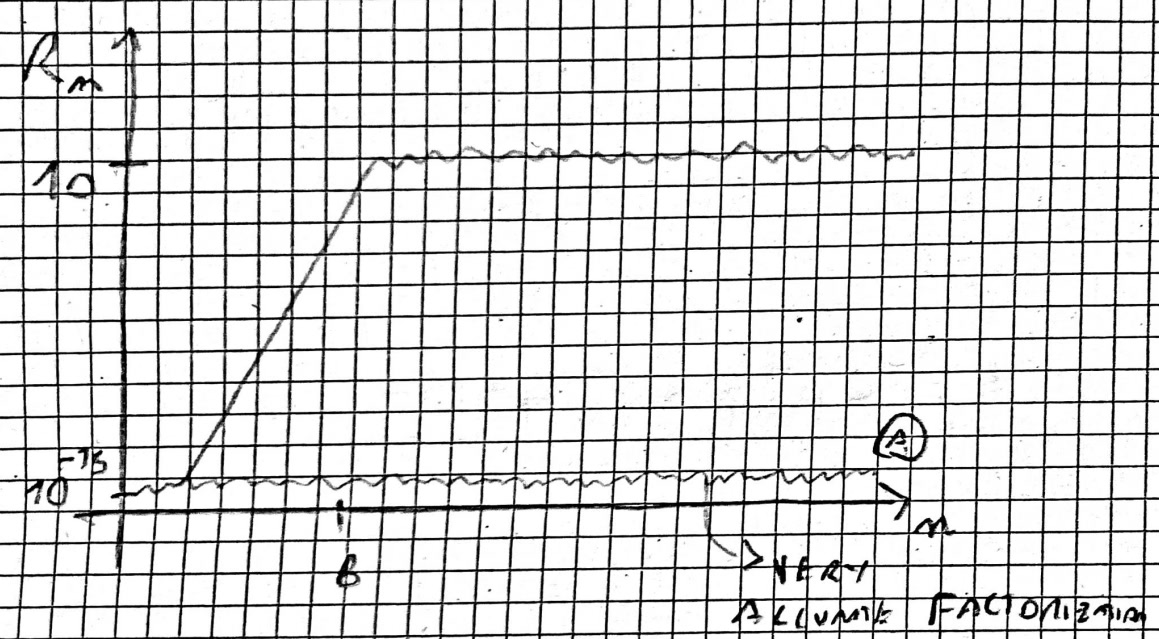
\includegraphics[width=0.8\textwidth]{images/accLU.png}
\end{center}
The reason is the problem, the Hilbert matrix is \textbf{ill positioned problem}. The method does not solve $Ax=b$, but retrieves the solution of the \textbf{perturbated system}:
$$
(A+\underlabel{\delta A}{$\mathbb{R}^{n\times n}$})(x+\delta x)=b+\underlabel{\delta b}{$\mathbb{R}^n$}
$$
$\delta b$ and $\delta A$ are perturbation on the data, matlab is computing the exact solution, but due to point floating point we will have a solution perturbation $\delta x$. We would like that for small perturbation on the data we get small perturbation on the problem (\textbf{well positioned problems}). Let the perturbated solution be
$$
\tilde{x}=x+\delta x
$$
Starting from $\delta A=0$, we want to relate the two perturbations:
$$\frac{||\delta A||}{||A||}\qquad\frac{||\delta b||}{||b||}$$
We must firstly introduce some lemmas.

\subsubsection{Lemmas}
\begin{enumerate}[1)]
    \item Let $B\in\mathbb{R}^{n\times n}$ be a spd matrix. Then it holds
    $$
    \lambda_{\min}(B)\leq\frac{x^TBx}{x^Tx}\leq\lambda_{\max}(B)\qquad\forall\,\,x\neq 0\in\mathbb{R}^n
    $$
    There $\lambda$'s are the eigenvalues.
    \item Let $A$ be a nonsingular matrix. Then $A^TA$ is spd
\end{enumerate}

\subsubsection{Perturbations relation}
Starting from $\delta A=0$, we want to relate the two perturbations:
$$\frac{||\delta A||}{||A||}\qquad\frac{||\delta b||}{||b||}$$
\begin{itemize}
    \item First step, we subtract term by term the exact system $Ax=b$ from the perturbated one $(A+0)(x+\delta x)=b+\delta b$:
    $$
    A\delta x = \delta b
    $$
    Consider the L2-norm (euclidean norm $||w||^2=w^Tw$):
    $$
    ||A\delta x||^2 = ||\delta b||^2\rightarrow
    (A\delta x)^T(A\delta x)=||\delta b||^2\rightarrow
    \delta x^TA^TA\delta x=||\delta b||^2
    $$
    From the lemma 2 $A^TA$ is spd, so we can apply lemma 1 with $B=A^TA$
    $$
    \lambda_{\min}(A^TA)\delta x^T\delta x\leq
    \delta x^TA^TA\delta x=||\delta b||^2\leq
    \lambda_{\max}(A^TA)\delta x^T\delta x
    $$
    With $\delta x^T\delta x=||\delta x||^2$. Consider only the left part of the inequality:
    $$
    \lambda_{\min}(A^TA)||\delta x||^2\leq||\delta b||^2
    $$
    $$
    ||\delta x||\leq
    \frac{
        ||\delta b||
    }{
        \sqrt{\lambda_{\min}(A^TA)}
    }
    $$
    \item As the next step consider
    $$
    ||Ax||^2=||b||^2
    $$
    Similar reasoning:
    $$
    \lambda_{\min}(A^TA)x^Tx\leq
    x^TA^Ax=(Ax)^TAx=||b||^2\leq
    \lambda_{\max}(A^TA)x^Tx
    $$
    With $x^Tx=||x||^2$. Consider only the right part of the inequality:
    $$
    ||b||\leq\sqrt{\lambda_{\max}(A^TA)}||x||
    $$
    $$
    \frac{1}{||x||}\leq\frac{\sqrt{\lambda_{\max}(A^TA)}}{||b||}
    $$
    \item We put everything together. As both inequalities are all positive quantities, we can combine them considering:
    $$
    \begin{cases}
        a\leq b\\
        c\leq d\\
    \end{cases}
    \rightarrow ab\leq cd
    $$
    \begin{LARGE}        
        $$
        \frac{||\delta x||}{||x||}\leq
        \underlabel{
            \sqrt{\frac{
                \lambda_{max}(A^TA)
            }{\lambda_{min}(A^TA)}}
        }{$K(A)\geq 1$ condition number}    
        \frac{||\delta b|}{||b||}
        $$
    \end{LARGE}

    The condition number can only amplify, a small perturbation on the data will be small as well if the condition number is almost 1 (well conditioned problem), but if the condition number is very large this relationship does not hold (ill conditioned problem, just like for Hilbert)
\end{itemize}

\subsubsection{Condition number}
$$
K(A)=||A||\cdot||A^{-1}||
$$
A norm of a matrix has 3 possible definitions
\begin{itemize}
    \item \textbf{Norm one}, maximum of the sum by columns
    \begin{center}
        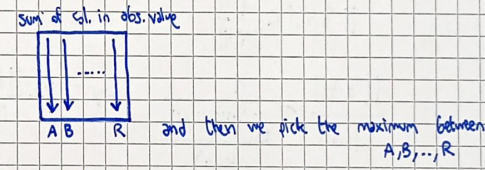
\includegraphics[width=0.8\textwidth]{images/normone.png}
    \end{center}
    $$||A||_1=\max_j\sum_{i=1}^n|a_{ij}|$$
    $$K(A)=||A||_1\cdot||A^{-1}||_1$$
    \item \textbf{Infinity norm}, first compress horizontally, then compress vertically, like dual of before
    $$||A||_\infty=\max_i\sum_{j=1}^n|a_{ij}|$$
    $$K(A)=||A||_\infty\cdot||A^{-1}||_\infty$$
    \item \textbf{2-norm or Spectral norm}, spectrum of a matrix is the collection of the eigenvalues
    $$
    ||A||_2=\sqrt{\lambda_{\max}(A^TA)}
    $$
    From before, we found that:
    $$
    K(A)=\sqrt{\frac{
        \lambda_{max}(A^TA)
    }{\lambda_{min}(A^TA)}}=||A||_2||A^{-1}||_2
    $$
    So before we found a particular condition number:
    $$K_2(A)=||A||_2||A^{-1}||_2$$
    \begin{itemize}
        \item A special case, if $A$ is symmetric ($A=A^T$), so $A^TA=A^2$
        $$
        \lambda_{\max}(A^2)=[\lambda_{\max}(A)]^2
        $$
        And
        $$
        ||A||_2=\lambda_{\max}(A)
        $$
        $$
        K_2(A)=\frac{\lambda_{\max}(A)}{\lambda_{\min}(A)}
        $$
    \end{itemize}
\end{itemize}
In matlab $cond(A)$ for 2-norm, $condest(A_sparse)$ for 1-norm

Now we can rewrite:
$$
\delta b = A\underlabel{(x+\delta x)}{perturbation $\tilde{x}$}-b=A\tilde{x}-b=-\tilde{r}
$$
We get the residual

\subsubsection{Perturbation on the matrix A}
What if $\delta A\neq 0$? If $||\delta A||||A^{-1}||<1$, we can:
$$
\frac{||\delta x||}{||x||}
\leq
\frac{K(A)}{1-K(A)\frac{||\delta A||}{||A||}}
\left[
    \frac{||\delta A||}{||A||}+\frac{||\delta b||}{||b||}
\right]
$$
From the hypothesis
$$
||\delta A||\cdot||A^{-1}||<1
\rightarrow
||\delta A||<\frac{1}{||A^{-1}||}
\rightarrow
\frac{||\delta A||}{||A||}<\frac{1}{||A||\cdot||A^{-1}||}
\rightarrow
K(A)\frac{||\delta A||}{||A||}<1
$$
Which means
$$
1-K(A)\frac{||\delta A||}{||A||}>0
$$
\textbf{In conclusion, before solving a problem check the condition number to see if it is ill conditioned or not. If condition number too huge problem}